%\vspace{0.2cm}
%\noindent{\it Example.}
\subsection{Example}

\begin{table}[bp]
%    \centering
	\caption{Evolution of Suspiciousness Scores for the Running Example in Figure~\ref{motiv_example} using RAPTOR~\citep{Alberto2011}.}
\hspace*{-20pt}
    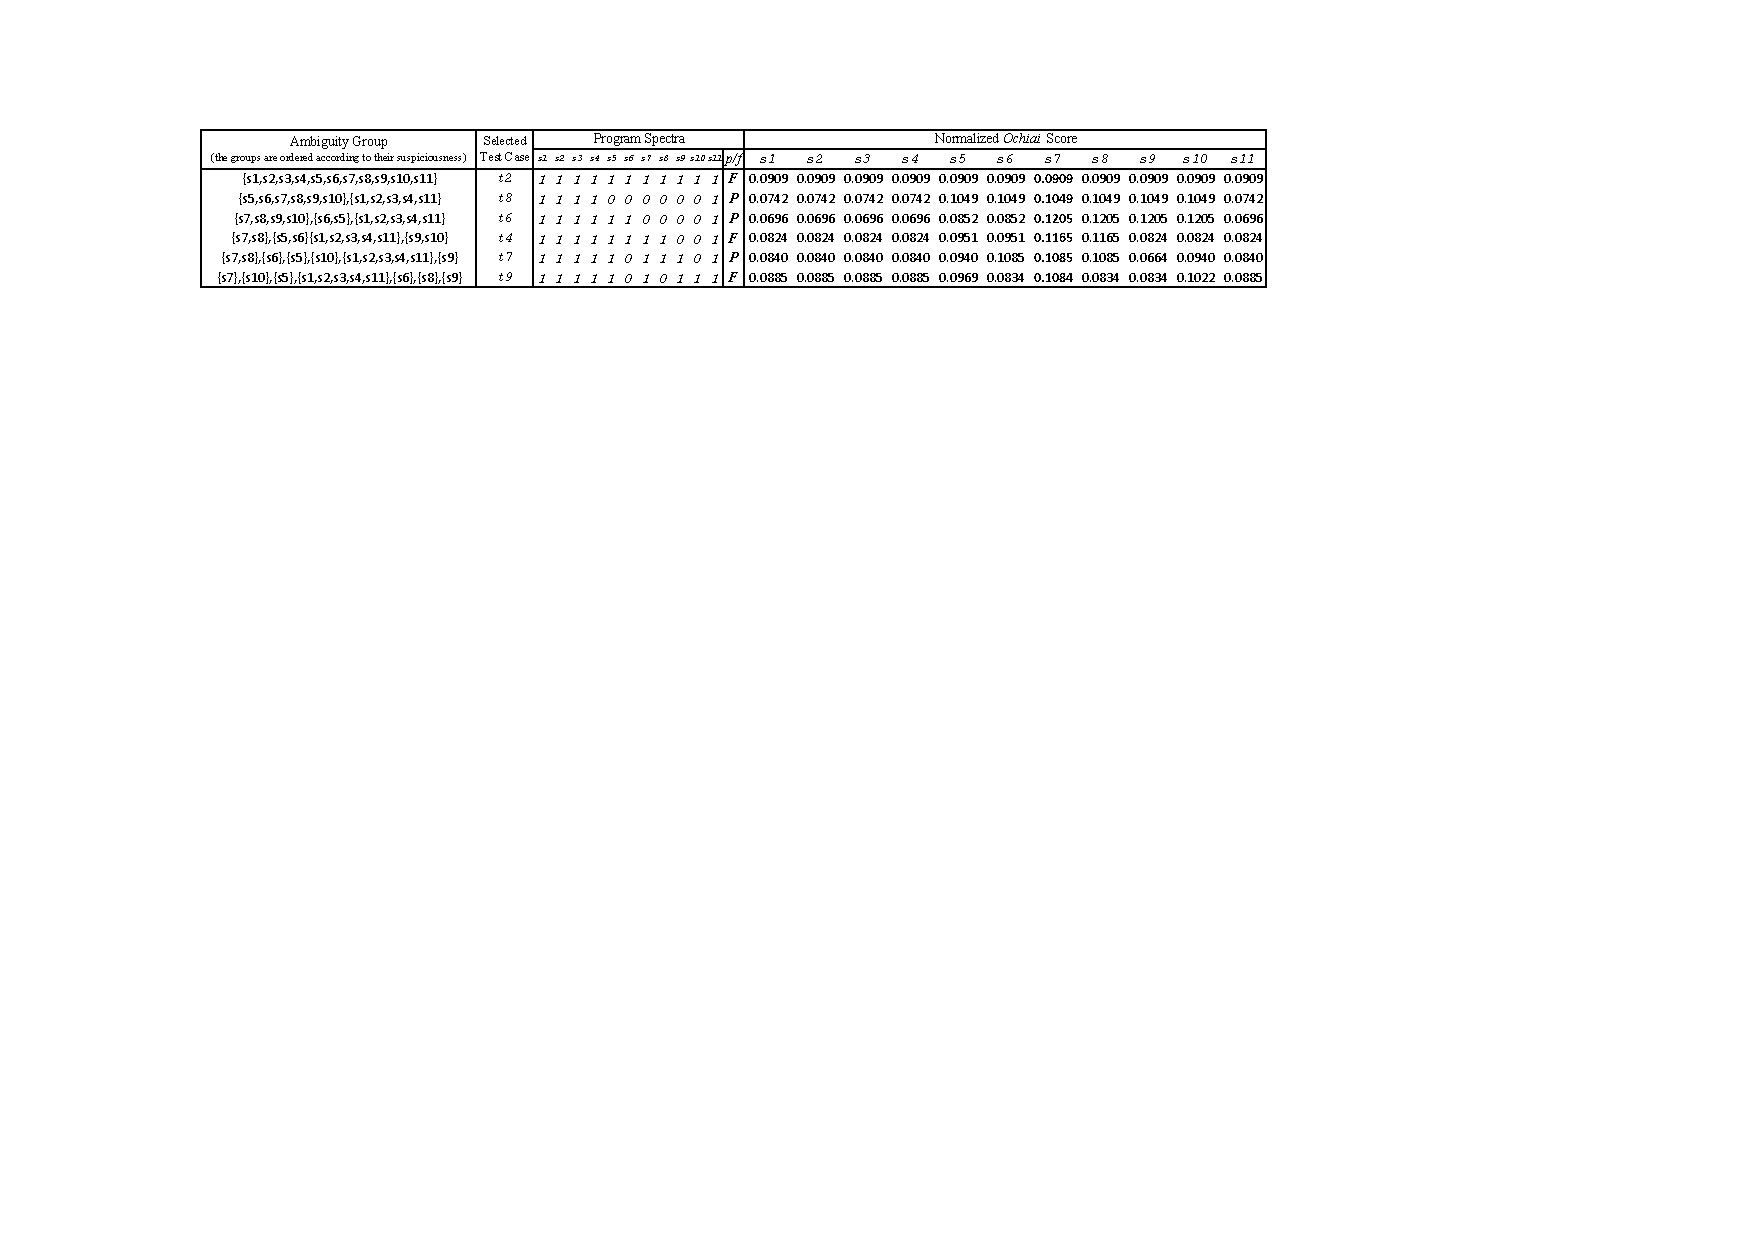
\includegraphics[width=13cm]{ag_table.pdf}
	%\vspace*{-16pt}
    \label{tab:ag_evo}
\end{table}


We describe step by step how \textsc{Dms} minimizes the number of test cases needed by {\em Ochiai} to locate
the fault in the running example in Figure~\ref{motiv_example} and Figure~\ref{tab:dms_evo}.

Since the example code snippet is quite small, there is no need to use a large number of initial test cases to bootstrap our trend analysis. %faulty element $s_{7}$ are ranked $1^{st}$ after selecting only a few traces using \textsc{Raptor}.
We set $w=1$ and thus only use one test case (in addition to $t_0$) for bootstrapping. In this example and our evaluation in Section~\ref{sec.experiment}, we use \textsc{Raptor}, one of the previously best techniques, in the bootstrapping process for better comparison.

Initially, users execute the program and expose a failure ($t_2$ in this example) in which all statements are covered.
Thus all statements get equal non-zero suspiciousness and constitute one suspicious group $g$ (cf.\ either Figure~\ref{tab:dms_evo} and Table~\ref{tab:ag_evo}). All non-zero suspicious groups compose a group set $G = \{g\}$.
{\sc Raptor} would then choose $t_8$ since $t_8$ has the maximum ambiguity reduction values, and present it to developers for labeling as either {\em pass} or {\em fail}).


After the bootstrapping stage, {\em Ochiai} updates the suspiciousness score for each statement based on the selected traces
and the existing suspicious group set are broken into \{$s_{1}$,$s_{2}$,$s_{3}$,$s_{4}$,$s_{11}$\} and \{$s_{5}$,$s_{6}$,$s_{7}$,$s_{8}$,$s_{9}$,$s_{10}$\} (cf.\ either Figure~\ref{tab:dms_evo} and Table~\ref{tab:ag_evo}), they are
called $g_{1}$ and $g_{2}$ respectively.
At this time, the trend for the statements in $g_{1}$ is {\bf\texttt{[+]}}, because the ranks of these statements change from 11 to 6, while the trend for the statements in $g_{2}$
is {\bf\texttt{[0]}}, because their ranks are still 11.
The corresponding time series of the statements in $g_{2}$ are:
$y_{0} = 0$ and $ y_{1} = 1$. Applying Equation \ref{eq:trend_metric}, we obtain the change potential of the trend of the program elements in $g_{2}$ as 1.


We now calculate $\mathcal{H}_{G}$ for the current suspicious group set $G=\{g_{1},g_{2}\}$ according to Equation \ref{eq:elem_potential}:

\[\mathcal{H}_{G} = \mathcal{W}_{g_{1}}^{2} + \mathcal{W}_{g_{2}}^{2}  = (\sum_{d \in g_{1}}{0})^{2} + (\sum_{d \in g_{2}}{1})^{2} = 36\].

Now there are 10 candidate traces: $\{t_{i} | 1\leq~i~\leq~12 \wedge i\notin\{2,8\}\}$ to be evaluated. We will use each candidate trace $t_{i}$ to
break ties in $G$ ($G \Leftarrow t_{i}$). Then we calculate the score that evaluates the breaking effect: $\mathcal{H}_{(G \Leftarrow t_{i})}$.

For example, when evaluating $t_6$, $t_{6}$ covers $s_{1}$,$s_{2}$,$s_{3}$,$s_{4}$,$s_{5}$,$s_{6}$ and $s_{11}$, thus breaks suspicious $g_{2}$
into \{$s_{5}$,$s_{6}$\} and \{$s_{7}$,$s_{8}$,$s_{9}$, $s_{10}$\}, let us call them $g_{21}$ and $g_{22}$ respectively.
Now, the score $\mathcal{W}_{g_{21}} = \frac{2}{6} \times \mathcal{W}_{g} = 2$, $\mathcal{W}_{g_{22}} = \frac{4}{6} \times 6 = 4$.
So if choosing $t_{6}$, the score for ($G\Leftarrow t_6$) is

\[\mathcal{H}_{(G \Leftarrow t_{6})} = \mathcal{W}_{g_{21}}^{2} + \mathcal{W}_{g_{22}}^{2} = 20\]
And the reduction is

\[\mathcal{H}_{G} - \mathcal{H}_{(G \Leftarrow t_{6})} = 36 - 20 = 16\].

In the same way, we evaluate all candidate traces and find that the reduction of $t_{6}$ is maximal, so we select $t_{6}$ as the next trace and ask a developer to manually label $t_{6}$.
The developer then labels it as {\em ``pass''}.  After adding newly labeled trace $t_{6}$ into the selected trace set $T_{\mathcal{S}}$, we recalculate the suspicious score
of all program elements according to the current selected trace set. After calculation, the normalized suspicious score of the elements in \{$s_{5}$,$s_{6}$\} reduced from 0.1049 to 0.0852 and their ranks remains the same. The suspicious scores of
the elements in \{$s_{7}$,$s_{8}$,$s_{9}$,$s_{10}$\} increase from 0.1049 to 0.1205 and thus their ranks rises from 6 to 4. After that, the trends of program elements are updated. For example, the trend of elements in \{$s_{1}$,$s_{2}$,$s_{3}$,$s_{4}$,$s_{13}$\} becomes ({\bf\texttt{[0]}}{\bf\texttt{[0]}}), the trend
of the statements in \{$s_{5}$,$s_{6}$\} becomes ({\bf\texttt{[+]}}{\bf\texttt{[0]}}) and those in \{$s_{7}$,$s_{8}$,$s_{9}$,$s_{10}$\} corresponds to ({\bf\texttt{[+]}}{\bf\texttt{[+]}}).


Note that right now \{$s_{7}$,$s_{8}$,$s_{9}$,$s_{10}$\} gets the highest change-potential score and thus can get more chances to be broken up.
As shown in Figure \ref{tab:dms_evo},
after three iterations,
\textsc{Dms} selects (\texttt{$t_{8}$}$\rightarrow$\texttt{$t_{6}$}$\rightarrow$\texttt{$t_{4}$}). In the next iteration, \textsc{Dms} chooses $t_{9}$ and breaks \{$s_{7}$,$s_{8}$\} and \{$s_{5}$,$s_{6}$\} which have greater change potentials and consequently ranks $s_7$ the highest. Overall, {\sc Dms} only requires user to manually label four additional traces (\texttt{$t_{8}$}$\rightarrow$\texttt{$t_{6}$}$\rightarrow$\texttt{$t_{4}$}$\rightarrow$\texttt{$t_{9}$}).

As a comparison, \textsc{Raptor} always chooses the test case that maximally reduces the overall sizes of groups of statements that have the spectrum records (i.e., Ambiguity Group Reduction, c.f.\ Section~\ref{subsubsec.dp}). As shown in Table~\ref{tab:ag_evo}, \textsc{Raptor} effectively selects the same test cases as {\sc Dms} in the first four iterations; however, it chooses $t_{7}$ in the next iteration to break \{$s_{1}$,$s_{2}$,$s_{3}$,$s_{4}$,$s_{9}$,$s_{10}$,$s_{11}$\} and \{$s_{5}$,$s_{6}$\}, and it takes one more iteration to rank $s_7$ the highest.
%Because breaking these groups can get maximal overall group size reduction.
It thus requires users to label five additional test cases besides $t_2$ (\texttt{$t_{8}$}$\rightarrow$\texttt{$t_{6}$}$\rightarrow$\texttt{$t_{4}$}$\rightarrow$\texttt{$t_{7}$}$\rightarrow$\texttt{$t_{9}$}).
